\documentclass[a4paper]{article}
\usepackage[utf8]{inputenc}
\usepackage[russian]{babel}
\usepackage[T2]{fontenc}
\usepackage[warn]{mathtext}
\usepackage{graphicx}
\usepackage{amsmath}
\usepackage{floatflt}
\usepackage[left=20mm, top=20mm, right=20mm, bottom=20mm, footskip=10mm]{geometry}


\graphicspath{ {images/} }
\usepackage{multicol}
\setlength{\columnsep}{2cm}


\begin{document}

\begin{titlepage}
	\centering
	\vspace{5cm}
	{\scshape\LARGE Московский физико-технический институт \par}
	\vspace{4cm}
	{\scshape\Large Лабораторная работа \par}
	\vspace{1cm}
	{\huge\bfseries Изучение дифракции света \par}
	\vspace{1cm}
	\vfill
\begin{flushright}
	{\large выполнила студент 653 группы ФФКЭ}\par
	\vspace{0.3cm}
	{\LARGE Давыдов Валентин}
\end{flushright}
	

	\vfill

% Bottom of the page
	Долгопрудный, 2018 г.
\end{titlepage}

\section{Цель работы}
Исследовать явления дифракции Френеля и Фраунгофера на щели, изучить влияние дифракции на разрешающую способность оптических приборов.

\section{В работе используются:}
\begin{itemize}
    \item оптическая скамья
    \item ртутная лампа
    \item монохроматор
    \item щели с регулируемой шириной
    \item рамка с вертикальной нитью
    \item двойная щель
    \item микроскоп на поперечных салазках с микрометрическим винтом
    \item зрительная труба
\end{itemize}

\section{Дифракция Френеля на щели}
\begin{enumerate}
    \item Схема установки для наблюдения дифракции Френеля на щели представлена на рис. 1. Дифракционная картина рассматривается с помощью микроскопа М, сфокусированного на некую плоскость наблюдения П. 
\begin{figure}[h]
    \centering
    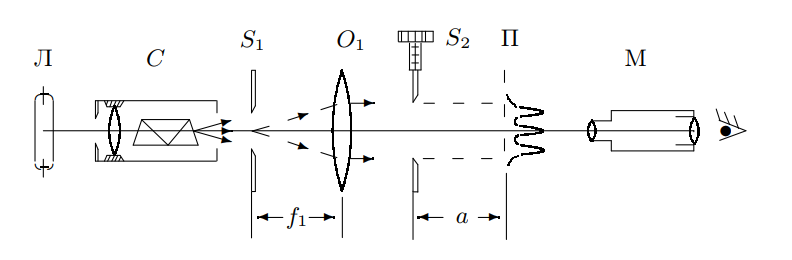
\includegraphics[width=15cm]{setup_frenel.PNG}
    \caption{Схема лабораторной установки для наблюдения дифракции Френеля}
    \label{fig:vac}
\end{figure}

\item Проведём настройку приборов, соберём установку. Наблюдаем дифракцию Френеля на щели - на ярком фоне изображения щели появляются узкие тёмные полосы, количество которых уменьшается по мере удаления микроскопа (дифракция в ближней волновой зоне) - фотографии представлены на рисунках 2 и 3.

\begin{figure}[h]
\begin{center}
\begin{minipage}[h]{0.45\linewidth}
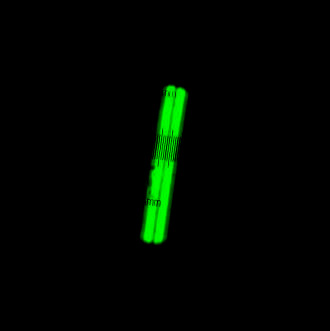
\includegraphics[width=1\linewidth]{fren_1.jpg}
\caption{1 тёмная полоса на фоне (дифракция Френеля)} %% подпись к рисунку
\label{ris:experimoriginal} %% метка рисунка для ссылки на него
\end{minipage}
\hfill 
\begin{minipage}[h]{0.45\linewidth}
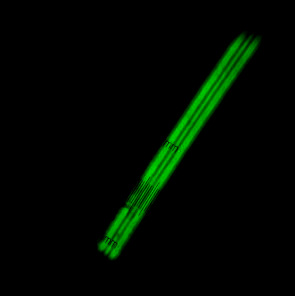
\includegraphics[width=1\linewidth]{fren_2.jpg}
\caption{2 тёмных полосы на фоне (дифракция Френеля)}
\label{ris:experimcoded}
\end{minipage}
\end{center}
\end{figure}

\begin{figure}[h]
    \centering
    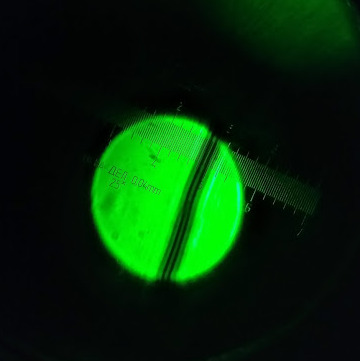
\includegraphics[width=7cm]{wire.jpg}
    \caption{Дифракция Френеля на препятствии}
    \label{fig:vac}
\end{figure}

\item Снимем зависимость координаты микроскопа от числа наблюдаемых полос, результаты занесём в таблицу 1.


\begin{table}[h]
    \centering
    \begin{center}
    \caption{Количество минимумов в зависимости от расстояния до плоскости наблюдения}
    \end{center}
    \vspace{0.1cm}
    \label{tab:my_label}
    \begin{tabular}{ |p{2.5cm}||p{0.5cm}|p{0.5cm}|p{0.5cm}|p{0.5cm}|p{0.5cm}|p{0.5cm}|p{0.5cm}|p{0.5cm}|}
 \hline
n тёмных полос & 0 & 1 & 2 & 3 & 4 & 5 & 6 & 7\\
 \hline
 $z$, мм & 52 & 50.8 & 51 & 51.2 & 51.3 & 51.4 & 51.5 & 51.6\\

 \hline
 
\end{tabular}
\end{table}


\item Сравним размер зон Френеля с измеренной шириной $b = 300$ мкм щели $S_2$. Для этого рассчитаем величину $2x_n=2\sqrt{zn\lambda}$($\lambda = 546.1$ нм) и построим график зависимости $2x_n = f(n)$ (рис. 5)
\begin{figure}[h]
    \centering
    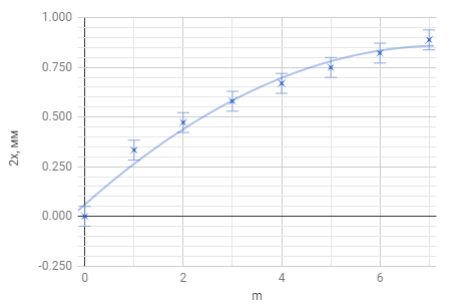
\includegraphics[width=12cm]{graph_fren.PNG}
    \caption{Зависимость ширины френелевских зон от номера n}
    \label{fig:vac}
\end{figure}

Видим, что ширина френелевских зон - величина порядка толщины щели.

\item Пронаблюдаем за дифракцией Френеля на проволоке. При удалении микроскопа от нити на её фоне всегда наблюдается чётное число тёмных дифракционных полос (светлый центр) - фото дифракции на препятствии представлено на рисунке 4.

\end{enumerate}

\section{Дифракция Фраунгофера на щели}

На значительном удалении от щели, когда ширина щели становится значительно меньше ширины первой зоны Френеля, изображение щели размывается и возникает дифракционная картина, называемая дифракцией Фраунгофера.

\begin{enumerate}
    \item Дифракцию Френеля и Фраунгофера можно наблюдать на одной и той же установке (поставив дополнительную линзу между щелью и плоскостью наблюдения). Дифракционная картина наблюдается в фокальной плоскости объектива $O_2$ (фокусное расстояние линзы $f_2 = 12.8$ см). Схема установки для наблюдения дифракции Фраунгофера на щели представлена на рис. 6. Фотография дифракционной картинцы представлена на рис. 8.
    
  \begin{figure}[h]
    \centering
    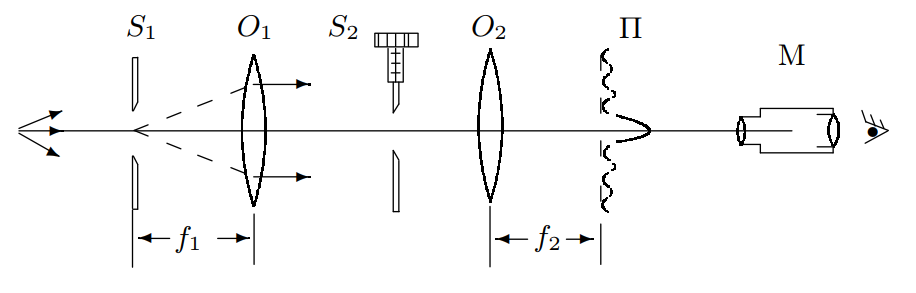
\includegraphics[width=12cm]{setup_fraunhofer.PNG}
    \caption{Схема лабораторной установки для наблюдения дифракции Фраунгофера на щели}
    \label{fig:vac}
\end{figure}  
    
    \item Настроим установку, с помощью винта поперечного перемещения микроскопа измерим координаты $X_m$ нескольких дифракционных минимумов от $-m$ до $m$. Занесём результаты в таблицу 2 (цена <<большого>> деления в 1/10 единицы верхней шкалы - 0.1 мм). 
    
    \begin{table}[h]
    \centering
    \begin{center}
    \caption{Координаты минимумов дифракционной картины}
    \end{center}
    \vspace{0.1cm}
    \label{tab:my_label}
    \begin{tabular}{ |p{2.5cm}||p{0.7cm}|p{0.5cm}|p{0.5cm}|p{0.5cm}|p{0.5cm}|p{0.7cm}|p{0.5cm}|p{0.5cm}|p{0.5cm}|p{0.5cm}|}
 \hline
m & -5 & -4 & -3 & -2 & -1 & 1 & 2 & 3 & 4 & 5\\
 \hline
 $x_m$, мм & 0.065 & 0.08 & 0.1 & 0.12 & 0.14 & 0.165 & 0.19 & 0.21 & 0.23 & 0.25\\

 \hline
 
\end{tabular}
\end{table}

\begin{figure}[h]
    \centering
    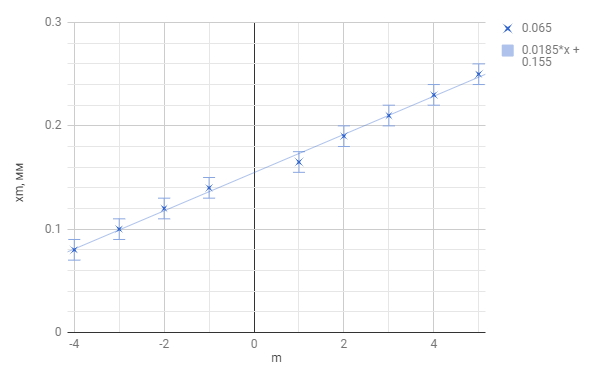
\includegraphics[width=12cm]{graph_frauh.PNG}
    \caption{Нахождение среднего расстояния между минимумами дифракционной картины Фраунгофера}
    \label{fig:vac}
\end{figure}

\item По углу наклона прямой определим среднее расстояние между соседними минимумами, рассчитаем ширину щели по формуле $b = \frac{\lambda f_2}{\tan} = 350$ мкм. Это значение практически совпадает с измеренным по микрометрическому винту ($b_0 = 300$ мкм)

\end{enumerate}

\begin{figure}[h]
\begin{center}
\begin{minipage}[h]{0.45\linewidth}
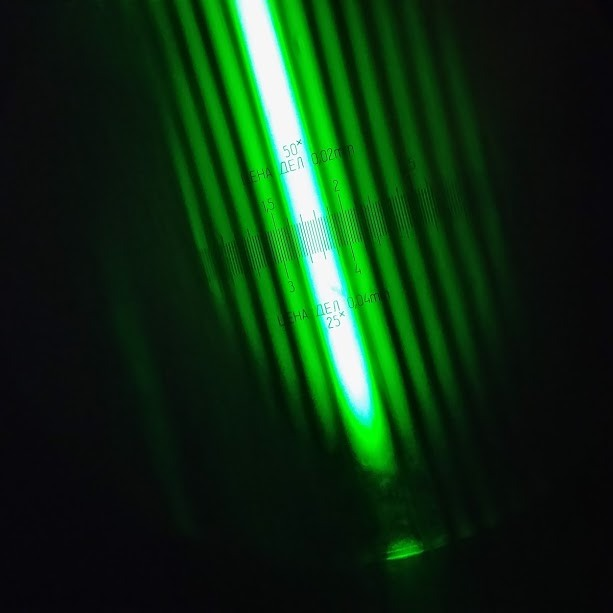
\includegraphics[width=1\linewidth]{frauh_1.jpg}
\caption{Дифракция Фраунгофера на одной щели} %% подпись к рисунку
\label{ris:experimoriginal} %% метка рисунка для ссылки на него
\end{minipage}
\hfill 
\begin{minipage}[h]{0.45\linewidth}
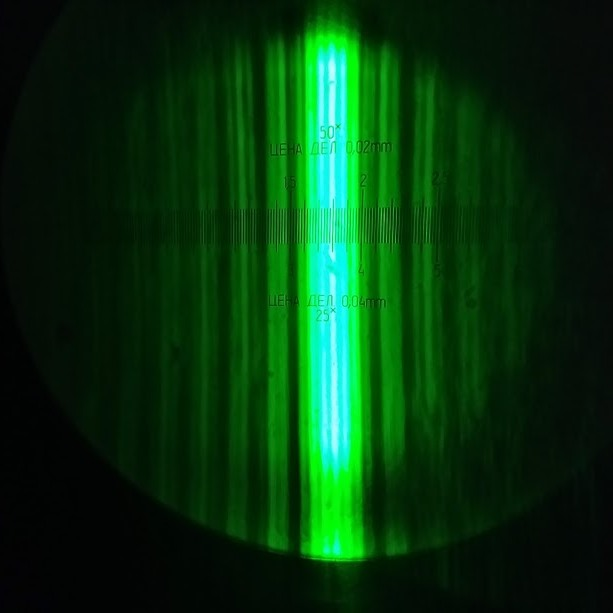
\includegraphics[width=1\linewidth]{frauh_2.jpg}
\caption{Дифракция Фраунгофера на двух щелях}
\label{ris:experimcoded}
\end{minipage}
\end{center}
\end{figure}

\section{Дифракция Фраунгофера на двух щелях}

\begin{enumerate}
     \item В установке для дифракции Фраунгофера для одной щели заменяем щель $S_2$ экраном Э с двумя щелями (рис. 10). В итоге получаем характерное распределение максимумов и минимумов (рис. 9 - фотография дифракционной картины Фраунгофера на двух щелях)


\item С помощью микрометрического винта поперечных салазок микроскопа определим координаты самых удалённых друг от друга полос, вычислим расстояние между ними ($\delta x = 0.18$ мм), между ними располагается 3 светлых промежутка. Расстояние между соседними минимумами в центральном максимуме равно $0.06$ мм. Тогда $d = \frac{f_2 \lambda}{\delta x} = 1.17$ мм. При этом расстояние между щелями, измеренное с помощью микроскопа, оказалось равным 1мм, значения совпадают.
\end{enumerate}

\newpage
\newpage

\section{Вывод}

В ходе работы было изучено явление дифракции света - дифракция Френеля на щели и на препятствии, дифракция Фраунгофера на одной и двух щелях.

\begin{itemize}
    \item При исследовании явления дифракции Френеля на щели убедились, что ширина зон Френеля примерно равна ширине щели
    
    \item При исследовании явления дифракции Фраунгофера на щели получили значение ширины щели, примерно равно измеренному непосредственно с помощью регулятора ширины щели:
    \begin{center}
        $b_0 = 300 $мкм \hspace{1cm} $b_f = 350$ мкм
    \end{center}
    
    \item При исследовании явления дифракции Фраунгофера на двух щелях было получено значение расстояния между щелями, примерно равное измеренному с помощью микроскопа:
    
    \begin{center}
        $d_0 = 1.17$ мм \hspace{1cm} $d_f = 1$ мм
    \end{center}
\end{itemize}


\end{document}
